
%summary of this section.
In this section, we report on the development and verification of a complex model translation that is used to compile high level embedded system models to C programs.
We start with some background on the mbeddr language, used to prescribe software for embedded systems. Afterwards we highlight the importance that this case study has for the embedded systems that perform critical functions and how our own tool SyVolt can contribute to the development of these.
Then we give an overview of the translation that performs the compilation of mbeddr models and we show one contract that a correct compilation must satisfy. Finally, we end the section with some discussion about the limits of the SyVolt contract language.

\subsection{Mbeddr: A programming Language for Embedded Systems}

% What is mbeddr and what it is used for.
Mbeddr is a set of domain-specific extensions to the C programming language \cite{Voelter:2012:MEC:2384716.2384767}. These linguistic extensions provide well known abstractions for programming embedded systems, namely, decision tables, components and interfaces, state machines, physical units, etc\ldots
Mbeddr has been used both academically and commercially \cite{Voelter2013,Voelter2014,mry_et_al:DR:2014:4543}.

% Components
Components are a useful abstraction because they allow the embedded system modeller to separate implementation from specification.
Mbeddr allows the modeller to declare interfaces, each with a set of operation signatures (\emph{specification}). Components then can declare provided or required ports. Each port is associated with an interface thus, if a component provides a port, it must implement the operations declared in the interface of that port (\emph{implementation}). 
Instances of components communicate between each other by invocating operations through their required ports. 
These instances of components are wired together by specifying, for each required port, what provided port - and by extension the component instance that provides that port - satisfies that requirement.
The implementation of operations can be done with pure C code, decision tables and state machines.

% Decision tables
Decision tables essentially abstract nested if statements. They are a useful abstraction because one can quickly express decision making based on a large number of variables. 

% State machines
State machines abstract switch/case statements. mbeddr also provides special syntactic constructs that allow the state machine to interact with its surrounding code, for instance, react to a invocation coming through a provided port. In mbeddr, state machines can only access local variables.

% Simple example and disclaimer that the simple example is not the case study.
To make the discussion of mbeddr concrete, we introduce a simple example but please notice that this example is not the case study. The case study is the compilation of any mbeddr model to C and not just this simple example.
Listing~\ref{code:simple_example_mbeddr} shows the textual syntax\footnote{Textual syntax is an abuse. mbeddr is developed in JetBrains Meta Programming System (MPS) and MPS uses a projectional editor where the user interacts directly with the abstract syntax tree of the model with no parsing involved.} of the mbeddr model.\cgg{I have to introduce keywords to this listing to make it prettier.}


\lstset{language=C, caption={Client/Server Example in mbeddr},label=code:simple_example_mbeddr} 
\begin{lstlisting}[float]
exported cs interface Client { 
  void client_process() 
} 

exported cs interface Server { 
  string server_process(string request) 
} 

exported component Client extends nothing { 
  provides Client clientInterface 
  requires Server clientcomp_serverInterface 
   
  void clientInterface_client_process() <= op clientInterface.client_process { 
    clientcomp_serverInterface.server_process("Hello"); 
  } runnable clientInterface_client_process 
} component ClientComponent 

exported component GoodServer extends nothing { 
  provides Server serverInterface 
  string serverInterface_server_process(string request) <= op serverInterface.server_process { 
    return request; 
  } runnable serverInterface_server_process 
} component GoodServer 

exported component BadServer extends nothing { 
  provides Server serverInterface 
  string serverInterface_server_process(string request) <= op serverInterface.server_process { 
    int32 x = 0; 
    while (x >= 0) { 
      x = x + 1; 
    } while 
    return request; 
  } runnable serverInterface_server_process 
} component BadServer 

instances instances { 
  instance ClientComponent clientComponent 
  instance GoodServer gserverComponent 
  instance BadServer bserverComponent 
  connect clientComponent.clientcomp_serverInterface to gserverComponent.serverInterface
}
\end{lstlisting}

This example consists of two interfaces, three components and one instance of each component:
\begin{compactdesc}
\item[Client and Server interfaces] define the operation signatures akin to how function prototypes are defined in C.
\item[Client component] provides the Client interface through a port called ``clientInterface'' and requires the Server interface through a port called ``clientcomp\_serverInterface''. The implementation of the operation ``client\_process'', declared in the Client interface is just the invocation of the ``server\_process'' operation of the Server interface through the ``clientcomp\_serverInterface'' port.
\item[GoodServer component] provides the Server interface and the implementation of the ``server\_process'' operation is just an echo.
\item[BadServer component] provides the Server interface and the implementation of the ``server\_process'' operation is an infinite loop. The reason for this odd choice off example will become clear in the next section.
\item[Instances] are declared for each component and the required ``clientcomp\_serverInterface'' port of the Client component instance is connected to the provided ``serverInterface'' port of the GoodServer component instance.
\end{compactdesc}


\subsection{Correct Embedded Systems}

% Embedded systems need to be reliable.
The main reason for us to choose this case study is that embedded systems need to be reliable: there are industry standards such as ISO-26262, DO-178B or IEC-61508 to help ensure reliability and there are critical embedded systems such as pacemakers \cite{mry_et_al:DR:2014:4543} that also need to be correct.

% Traditional development of reliable embedded systems
Traditionally, embedded systems are implemented in C code and reliability is ensured by a combination of testing and model checking. Testing only guarantees reliability in as far as the test cases go and because C is very expressive, C programs need to be abstracted in order to properly apply model checking techniques \cite{Ivancic2005}. 
The abstraction process is error prone and time consuming as is described in \cite{Corbett2000} and \cite{Ratiu:2012:LEE:2663689.2663692}.

% Mbeddr contribution to the reliable embedded systems development
Mbeddr represents an evolution of traditional embedded system development because it starts with abstractions that can be proven to be correct and then generates C code. Model checking techniques can be applied to Mbeddr models because they contain higher level information (e.g., a state machines or decision tables) whereas With plain C code, these abstractions need to be inferred from the C.

% how does mbeddr help ensure correct embedded systems
Mbeddr is integrated with the NuSMV~\cite{Cimatti2002} model checker to perform model checking of the state machines and with the Yices~\cite{Dutertre:cav2014} Satisfiability Modulo Theories (SMT) solver to check the consistency and completeness of the decision tables.

% properties vs contracts
It is important to distinguish two types of properties: properties that ensure that a given mbeddr model needs to satisfy; and properties that all mbeddr models need to satisfy. we will call the later type as contracts.
For instance, a property of the former type for the mbeddr model of the pacemaker system is that it never stops. A contract is for mbeddr models that have decision tables is that these must be consistent and complete \cite{Ratiu:2012:LEE:2663689.2663692}. A contract for mbeddr models that have state machines is that these are free of unreachable states and dead transitions.
Properties can be seen as contracts in the form of an implication ``if the model has a certain form, then\ldots'' so we will be focusing in contracts.

%the problems with mbeddr level of abstraction
As described in \cite{Ratiu:2012:LEE:2663689.2663692}, contracts checked at the mbeddr level can only be sound if the C code that is generated satisfies the same contracts as the mbeddr models. 
This is precisely the definition of correctness of the C code generation. 
In practice this correctness can be ensured by manual reviews of the code generation and automated testing.

%how can syvolt help to ensure reliability
SyVolt is a step towards ensuring the C code generation is correct automatically without having to perform these checks in the generated code, provided the appropriate contracts are described.
It allows the user to express contracts that relate the generated C constructions with the elements in the mbeddr model.
This is something that cannot be done by checking the generated C code alone as it requires the traceability information between the generated C code and the mbeddr model.

%example
For instance, in SyVolt it is possible to prove that the wiring of instances of components is always respected, i.e., when executing the C code, no instance will invoke a different operation than the one that is specified in the wiring scheme at the mbeddr level. This is an important contract as it ensures, for instance, that the Client component instance in our Client/Server example (see Listing~\ref{code:simple_example_mbeddr}) will never invoke the operation of the BadServer component instance.
To see how non trivial this contract can be, look at the wiring function \verb=client_wire= of the generated code from the Client/Server example shown in Listing~\ref{code:components_sample_c}.: the wiring in the C code is done by assignment the address of the required port operation to a function pointer that is part of the instance's runtime data.
For more complex examples, this becomes very difficult to inspect in the generated code.

\lstset{language=C, caption={Client/Server Example in mbeddr},label=code:components_sample_c} 
\begin{lstlisting}[float]
struct Client_i_t {
  void (*client_process)(void*);
};
struct Server_i_t {
  char* (*server_process)(char*,void*);
};

struct Client_c_t {
  void *client_serverI_port;
  Server_i_t *client_serverI_ops;
};
struct BadServer__cdata { uint8_t aMember; };
struct GoodServer__cdata { uint8_t aMember; };

static Server_i_t bserver_serverI_ops;
static Client_i_t client_clientI_ops;
static Server_i_t gserver_serverI_ops;

static BadServer_c_t bserver_inst;
static Client_c_t client_inst;
static GoodServer_c_t gserver_inst;

char* BadServer_serverI_server_process(char *request, void *_id) 
{
  BadServer_c_t *cid = ((BadServer_c_t *)(_id));
  int32_t x = 0;
  while (x >= 0){
    x = x + 1;
  }
  return request;
}

void Client_clientI_client_process(void *_id) 
{
  Client_c_t *cid = ((Client_c_t *)(_id));
  (*cid->client_serverI_ops->server_process)("Hello",cid->client_serverI_port);
}

char* GoodServer_serverI_server_process(char *request, void *_id) 
{
  GoodServer_c_t *cid = ((GoodServer_c_t *)(_id));
  return request;
}

static void init(void) 
{
  client_wire();
  gserver_wire();
  bserver_wire();
}

static inline void bserver_wire(void) 
{
  bserver_serverI_ops.server_process = &BadServer_serverI_server_process;
}
static inline void client_wire(void) 
{
  client_clientI_ops.client_process = &Client_clientI_client_process;
  client_inst.client_serverI_port = &gserver_inst;
  client_inst.client_serverI_ops = &gserver_serverI_ops;
}
static inline void gserver_wire(void) 
{
  gserver_serverI_ops.server_process = &GoodServer_serverI_server_process;
}
\end{lstlisting}


\subsection{Mbeddr to C Code Generation}

%small intro to this section
Listing~\ref{code:components_sample_c} already disclosed the generated C code for the Client/Server mbeddr model shown in Listing~\ref{code:simple_example_mbeddr}. However, we have not disclosed how, in general, is the C code generated from an mbeddr model.
The C code is generated with a model transformation specified between two metamodels: the source metamodel is the mbeddr metamodel and the target metamodel is the C metamodel.

\subsubsection{Source and Target Metamodels}

We present a simplified version of the mbeddr metamodel in Figure~\ref{fig:Moduleclassdiagram}:
\begin{compactdesc}
	\item[ImplementationModule] represents the root container of the mbeddr model. It is composed of InstanceConfigurations, AtomicComponents and ClientServerInterfaces. There are other kinds of interfaces but they are not relevant for our purposes.
	\item[ClientServerInterface] represents a set of Operations. An Operation represents a signature, with arguments and typing information. We omit these details to keep the discussion short. In Listing~\ref{code:simple_example_mbeddr} there are two ClientServerInterfaces - Client and Server - each with one Operation.
	\item[AtomicComponent] represents a component. It has Ports, which can be ProvidedPorts or RequiredPorts, and Executables. Executables essentially represent an operation implementation. OperationTriggers define which port and operation the executable is implementing. In Listing~\ref{code:simple_example_mbeddr}, the GoodServer component has one provided port, named \verb=serverInterface=, and one executable named \verb=serverInterface_server_process= that is executed whenever the operation \verb=server_process= is invoked through the port \verb=serverInterface=. We have omitted the body of the Executable.
	\item[InstanceConfiguration] represent the runtime configuration of the component instances. It is comprised of ComponentIntance declarations and AssemblyConnectors. AssemblyConnectors allow the modeller to establish the connections between required and provided ports, and the instances.  In Listing~\ref{code:simple_example_mbeddr}, the InstanceConfiguration has three instances and one AssemblyConnector that connects the RequiredPort \verb=clientcomp_serverInterface= of the \verb=clientComponent= instance to the ProvidedPort \verb=serverInterface= of the \verb=gserverComponent= instance.
This means that, the required port invocation \verb=server_process("Hello")= in the \verb=Client= will be handled by the \verb=GoodServer=.
\end{compactdesc}

\begin{figure}
\begin{center}
  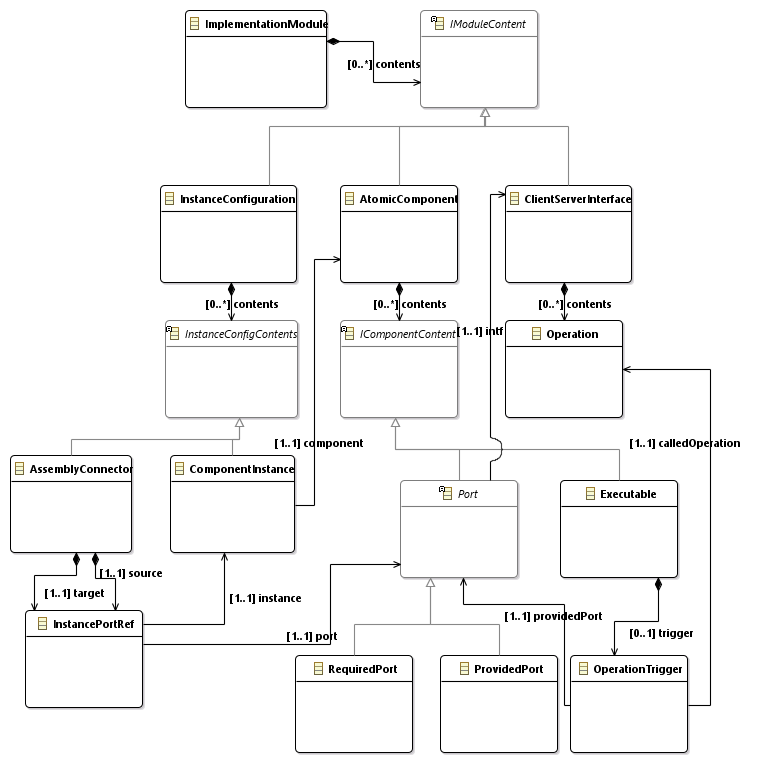
\includegraphics[width=0.48\textwidth]{figures/Moduleclassdiagram}
  \caption{Simplified mbeddr metamodel. \cgg{This picture needs to be compressed.}}
  \label{fig:Moduleclassdiagram}
\end{center}
\end{figure}

The simplified version of the C metamodel is shown in Figure~\ref{fig:CModelclassdiagram}. 
We have included only the concepts that are relevant for the contract we prove in this case study.
A C model has multiple compilation units, which we call ImplementationModules. An ImplementationModule has TypeDefs, StructDeclarations, FunctionPrototypes, Functions and GlobalVariableDeclarations.
In Listing~\ref{code:components_sample_c}, the ImplementationModule has five StructDeclarations, six GlobalVariableDeclarations and seven Functions.
The \verb=Client_i_t= structure has a CFunctionPointerStructMember named \verb=client_process=. The remaining concepts should be familiar to the reader\cgg{Should I give more details about the C or can I assume that they know C?}.

\begin{figure}
\begin{center}
  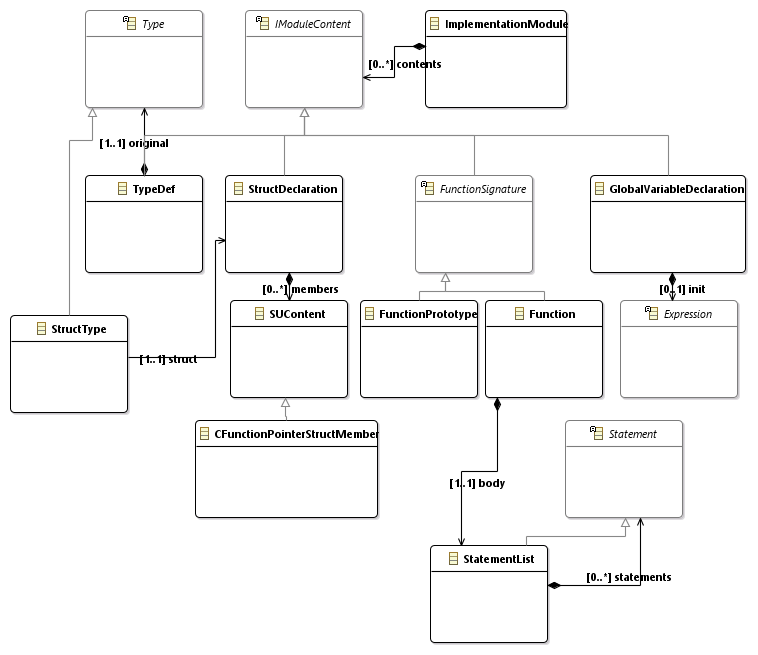
\includegraphics[width=0.48\textwidth]{figures/CModelclassdiagram}
  \caption{Simplified C metamodel. \cgg{This picture needs to be compressed.}}
  \label{fig:CModelclassdiagram}
\end{center}
\end{figure}










































